\documentclass{article}
\usepackage{geometry}
\usepackage{titling}
\usepackage{hyperref}
\usepackage{amsmath}
\usepackage{amssymb}
\usepackage{graphicx}

\geometry{
  a4paper,
  total = {170mm, 257mm},
  left = 20mm,
  top = 20mm,
}
\graphicspath{ {./images/} }

\title{Trabajo práctico N° 1}
\author{Emanuel Nicolás Herrador}
\date{Marzo 2025}

\makeatletter
\def\@maketitle{%
  \newpage
  \null
  \vskip 1em%
  \begin{center}%
  \let \footnote \thanks
    {\LARGE \@title \par}%
    \vskip 1em%
    {\large \@date}%
  \end{center}%
  \par
  \vskip 1em}
\makeatother

\begin{document}

\maketitle

\noindent\begin{tabular}{@{}ll}
	Estudiante & \theauthor \\
\end{tabular}

\section*{Ejercicio 1}
La herramienta de LTSA se puede encontrar dentro de la carpeta \textit{tools} en el repositorio.

\section*{Ejercicio 2}
El capítulo $1$ es el resumen de la clase $1$, mientras que el $2$ y $3$ están en el de la segunda clase.

\section*{Ejercicio 3}
\subsection*{Meeting}
\begin{verbatim}
  MEETING = (hello -> converse -> goodbye -> STOP).
\end{verbatim}

\subsection*{Job}
\begin{verbatim}
  JOB = (arrive -> work -> leave -> JOB).
\end{verbatim}

\subsection*{Movie}
\begin{verbatim}
  MOVIE = (ahead -> (
             left -> STOP
            |right -> MOVIE
          )).
\end{verbatim}

\subsection*{Game}
\begin{verbatim}
  GAME = (tree -> lose -> GAME
         |{one, two} -> WIN
         ),
  WIN = (win -> GAME).
\end{verbatim}

\subsection*{Four Tick}
\begin{verbatim}
  FOURTICK (N=4) = TICK[N],
  TICK[i:1..N] = (when(i == 1) tick -> STOP 
                 |when(i != 1) tick -> TICK[i-1]
                 ).
\end{verbatim}

\subsection*{Double}
\begin{verbatim}
  DOUBLE (N=3) = (in[i:1..N] -> out[i] -> DOUBLE).
\end{verbatim}

\subsection*{Person}
\begin{verbatim}
  PERSON = (weekend -> sleep -> {play, shop} -> PERSON
           |weekend -> sleep -> work -> PERSON
           ).
\end{verbatim}

\section*{Ejercicio 4}
\begin{verbatim}
  VARIABLE (N=2) = VAR[0],
  VAR[i:0..N] = (read[i] -> VAR[i]
                |write[j:0..N] -> VAR[j]
                ).
\end{verbatim}

\section*{Ejercicio 5}
\begin{verbatim}
  BITSTABLE (N=1) = BIT[N],
  BIT[i:0..1] = (trigger -> [i] -> BIT[!i]).
\end{verbatim}

\section*{Ejercicio 6}
\begin{verbatim}
  WATER_LVL (N=5) = LEVEL[5],
  LEVEL[i:0..9] = (when(i < 9) increment -> CHANGE_LEVEL[i + 1]
                  |when(i > 0) decrement -> CHANGE_LEVEL[i - 1]
                  ),
  CHANGE_LEVEL[i:0..9] = (when(i < 2) bajo -> LEVEL[i]
                         |when(i > 8) alto -> LEVEL[i]
                         |when(i >= 2 && i <= 8) normal -> LEVEL[i]
                         ).
\end{verbatim}

\section*{Ejercicio 7}
\begin{verbatim}
  DRINK_MACHINE = MONEY[0],
  MONEY[i:{[0], [5], [10]}] = (insert[j:{[5], [10], [20]}] -> CHECK[i + j]),
  CHECK[i:{[5], [10]}] = MONEY[i],
  CHECK[i:{[15], [20], [25], [30]}] = (drink -> RETURN[i - 15]),
  RETURN[0] = MONEY[0],
  RETURN[i:{[5], [10], [15]}] = (when(i == 5) return5 -> RETURN[i - 5]
                                |when(i >= 10) return10 -> RETURN[i - 10]
                                ).
\end{verbatim}

\section*{Ejercicio 8}
\begin{verbatim}
  const MIN = 88
  const MAX = 108 
  range T = MIN..MAX 

  RADIO = (on -> RADIO[MAX]),
  RADIO[i:T] = (off -> RADIO 
               |reset -> RADIO[MAX]
               |scan -> SCAN[i]
               ),
  SCAN[i:T] = (when(i == MIN) failed_scan -> RADIO[i]
              |when(i > MIN) try_another_scan -> SCAN[i - 1]
              |successfull_scan -> RADIO[i]
              ).
\end{verbatim}

\section*{Ejercicio 9}
Se comportan de la misma manera porque en la composición se comparte la acción $b$.
Por ello, es allí donde $P$ y $Q$ se sincronizan.
Aunque puedan realizar las transiciones en paralelo de $a$ y $c$, ambos deben hacer $b$ en conjunto (i.e., se establece que $a$ y $c$ deben ser realizadas antes, aunque en cualquier orden, y las dos deben estar hechas para hacer $b$).

Dado esto, se explica que tengan el mismo comportamiento.
También puede verse en LTSA.

\section*{Ejercicio 10}
\begin{verbatim}
  const N = 5 
  range T = 0..N 

  DIRECTOR = (opening -> closing -> DIRECTOR).

  GATE = (open -> GATE_ON),
  GATE_ON = (close -> GATE
            |person -> GATE_ON
            ).

  CONTROL = (opening -> open_doors -> CONTROL_ON[0]),
  CONTROL_ON[i:T] = (when(i < N) arrival -> CONTROL_ON[i + 1]
                    |when(i > 0) exit -> CONTROL_ON[i - 1]
                    |closing -> close_arrivals -> CONTROL_END[i]
                    ),
  CONTROL_END[i:T] = (when(i == 0) close_exits -> CONTROL
                    |when(i > 0) exit -> CONTROL_END[i - 1]
                    ).

  ||MUSEUM = (DIRECTOR || CONTROL || {east, west}:GATE)
            /{open_doors/{east, west}.open,
              arrival/east.person,
              exit/west.person,
              close_arrivals/east.close,
              close_exits/west.close}.
\end{verbatim}

\section*{Ejercicio 11}
\begin{figure}[ht]
	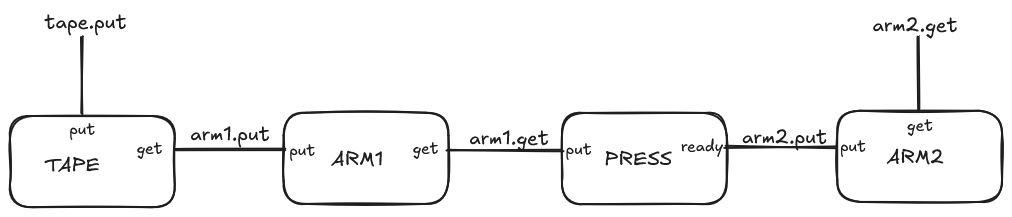
\includegraphics[width=0.8\textwidth]{01-11.png}
	\centering
\end{figure}
\begin{verbatim}
  BUFFER (BN=2) = BUFFER[0],
  BUFFER[i:0..BN] = (when(i < BN) put -> BUFFER[i+1]
                    |when(i > 0) get -> BUFFER[i-1]
                    ).

  PRESS = (put -> press -> ready -> PRESS).

  ||CELL = (tape:BUFFER(3) || arm[1..2]:BUFFER(1) || press:PRESS)
           /{arm[1].put/tape.get,
             arm[1].get/press.put,
             arm[2].put/press.ready}.
\end{verbatim}

\pagebreak
\section*{Ejercicio 12}
\begin{figure}[ht]
	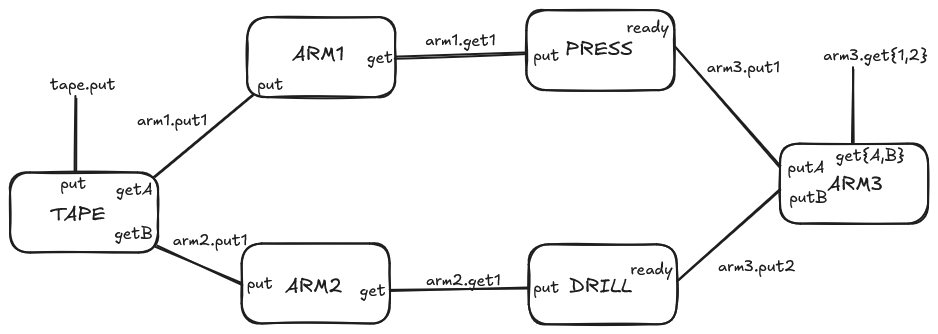
\includegraphics[width=0.8\textwidth]{01-12.png}
	\centering
\end{figure}
\begin{verbatim}
  /* Buffer with order */ 
  BUFF (NT=2) = (put[obj:1..NT] -> get[obj] -> BUFF).
  ||BUFFER (BN=2, NT=2) = ([1..BN]:BUFF(NT))
                          /{put[obj:1..NT]/[1].put[obj],
                            [i:2..BN].put[obj:1..NT]/[i-1].get[obj],
                            get[obj:1..NT]/[BN].get[obj]}
                          @{put[obj:1..NT], get[obj:1..NT]}.

  MACHINE = (put -> action -> ready -> MACHINE).

  ||CELL = (tape:BUFFER(3, 2) || arm[1..2]:BUFF(1) || arm[3]:BUFF(2)
                              || {press, drill}:MACHINE)
           /{arm[1].put[1]/tape.get[1],
            arm[2].put[1]/tape.get[2],
            arm[1].get[1]/press.put,
            arm[2].get[1]/drill.put,
            arm[3].put[1]/press.ready,
            arm[3].put[2]/drill.ready}.
\end{verbatim}

\section*{Ejercicio 13}
\begin{figure}[ht]
	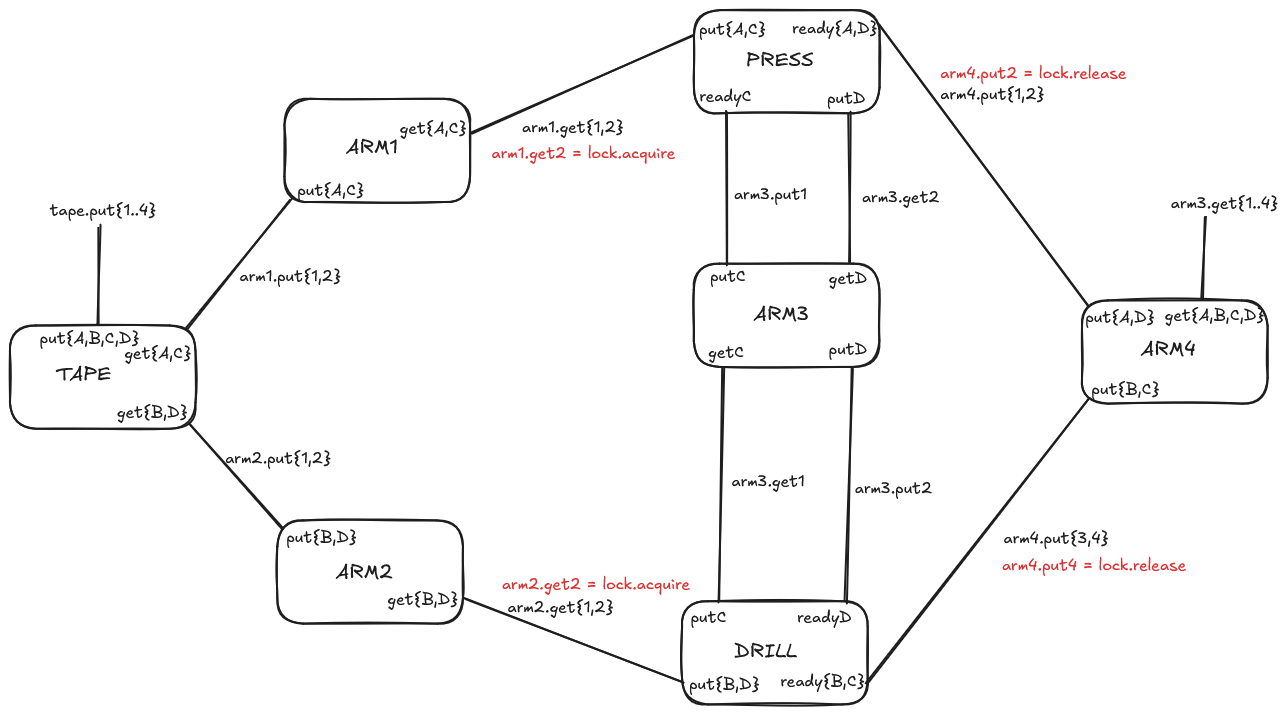
\includegraphics[width=0.9\textwidth]{01-13.png}
	\centering
\end{figure}
\begin{verbatim}
  /* Buffer with order */
  BUFF (NT=2) = (put[obj:1..NT] -> get[obj] -> BUFF).
  ||BUFFER (BN=2, NT=2) = ([1..BN]:BUFF(NT))
                          /{put[obj:1..NT]/[1].put[obj],
                            [i:2..BN].put[obj:1..NT]/[i-1].get[obj],
                            get[obj:1..NT]/[BN].get[obj]}
                          @{put[obj:1..NT], get[obj:1..NT]}.

  LOCK = (acquire -> release -> LOCK).

  MACHINE (NT=3) = (put[obj:1..NT] -> action -> ready[obj] -> MACHINE).

  ||CELL = (tape:BUFFER(3, 4) || arm[1..3]:BUFF(2) || arm[4]:BUFF(4)
                              || {press, drill}:MACHINE(3) || lock:LOCK)
           /{arm[1].put[i:1..2]/tape.get[i*2-1],
             arm[2].put[i:1..2]/tape.get[i*2],
             arm[1].get[i:1..2]/press.put[i],
             arm[2].get[i:1..2]/drill.put[i],
             arm[4].put[i:1..2]/press.ready[i*2-1],
             arm[4].put[i:3..4]/drill.ready[2*i-5],
             
             arm[3].put[1]/press.ready[2],
             arm[3].put[2]/drill.ready[2],
             arm[3].get[1]/drill.put[3],
             arm[3].get[2]/press.put[3],

             arm[1..2].get[2]/lock.acquire,
             arm[4].put[{[2], [4]}]/lock.release
            }.
\end{verbatim}

\end{document}
